\chapter{Конструкторская часть}

\section{Схемы алгоритмов}

На вход каждому из алгоритмов подаются матрицы A и B, а также числа N, M и K. Предполагается, что входные данные корректны: N, M и K больше 0, A размером N на M, B размером M на K.

\begin{figure}[h!]
	\centering
	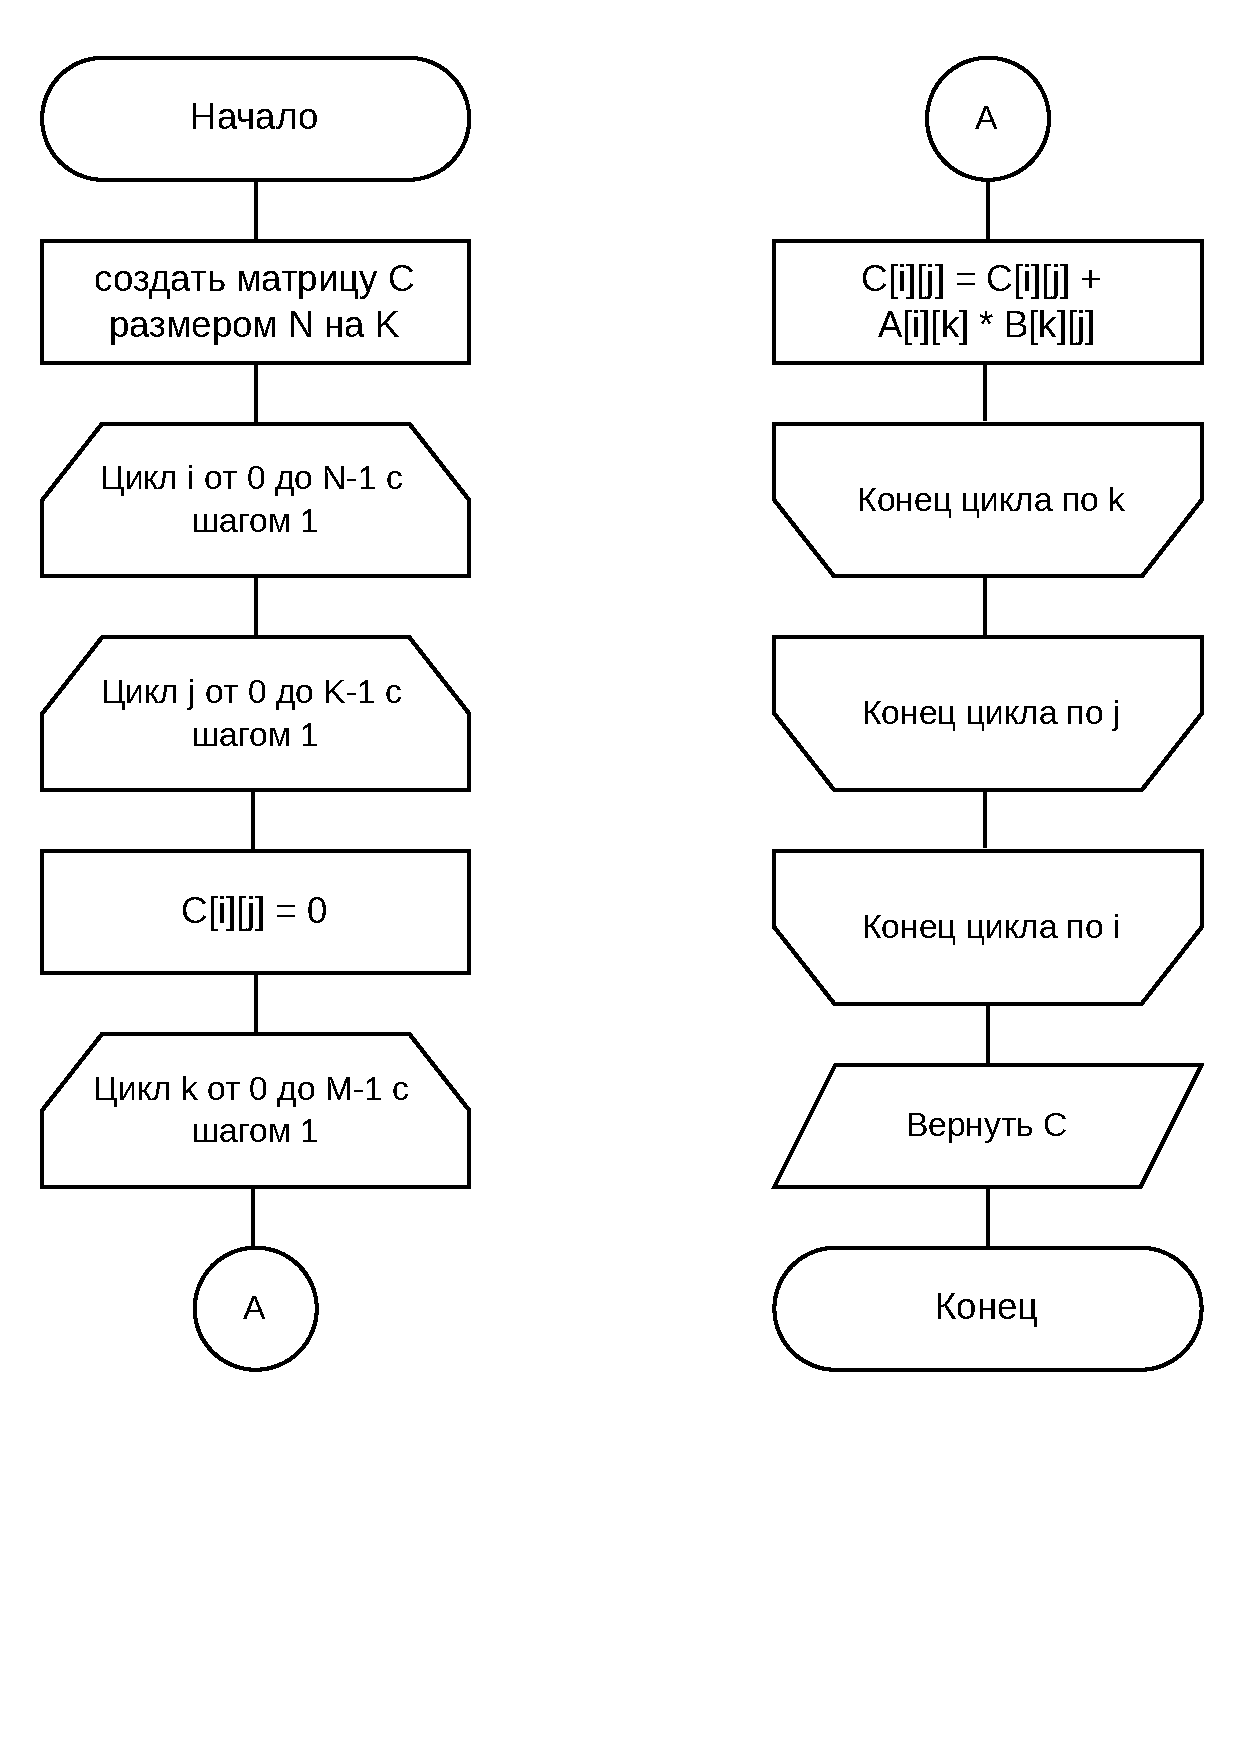
\includegraphics[height=0.6\textheight, width=0.6\textwidth]{tex_parts/scheme1.pdf}
	\caption{\label{fig:st}Схема стандартного алгоритма нахождения прозведения матриц}
\end{figure}

\clearpage

\begin{figure}[h!]
	\centering
	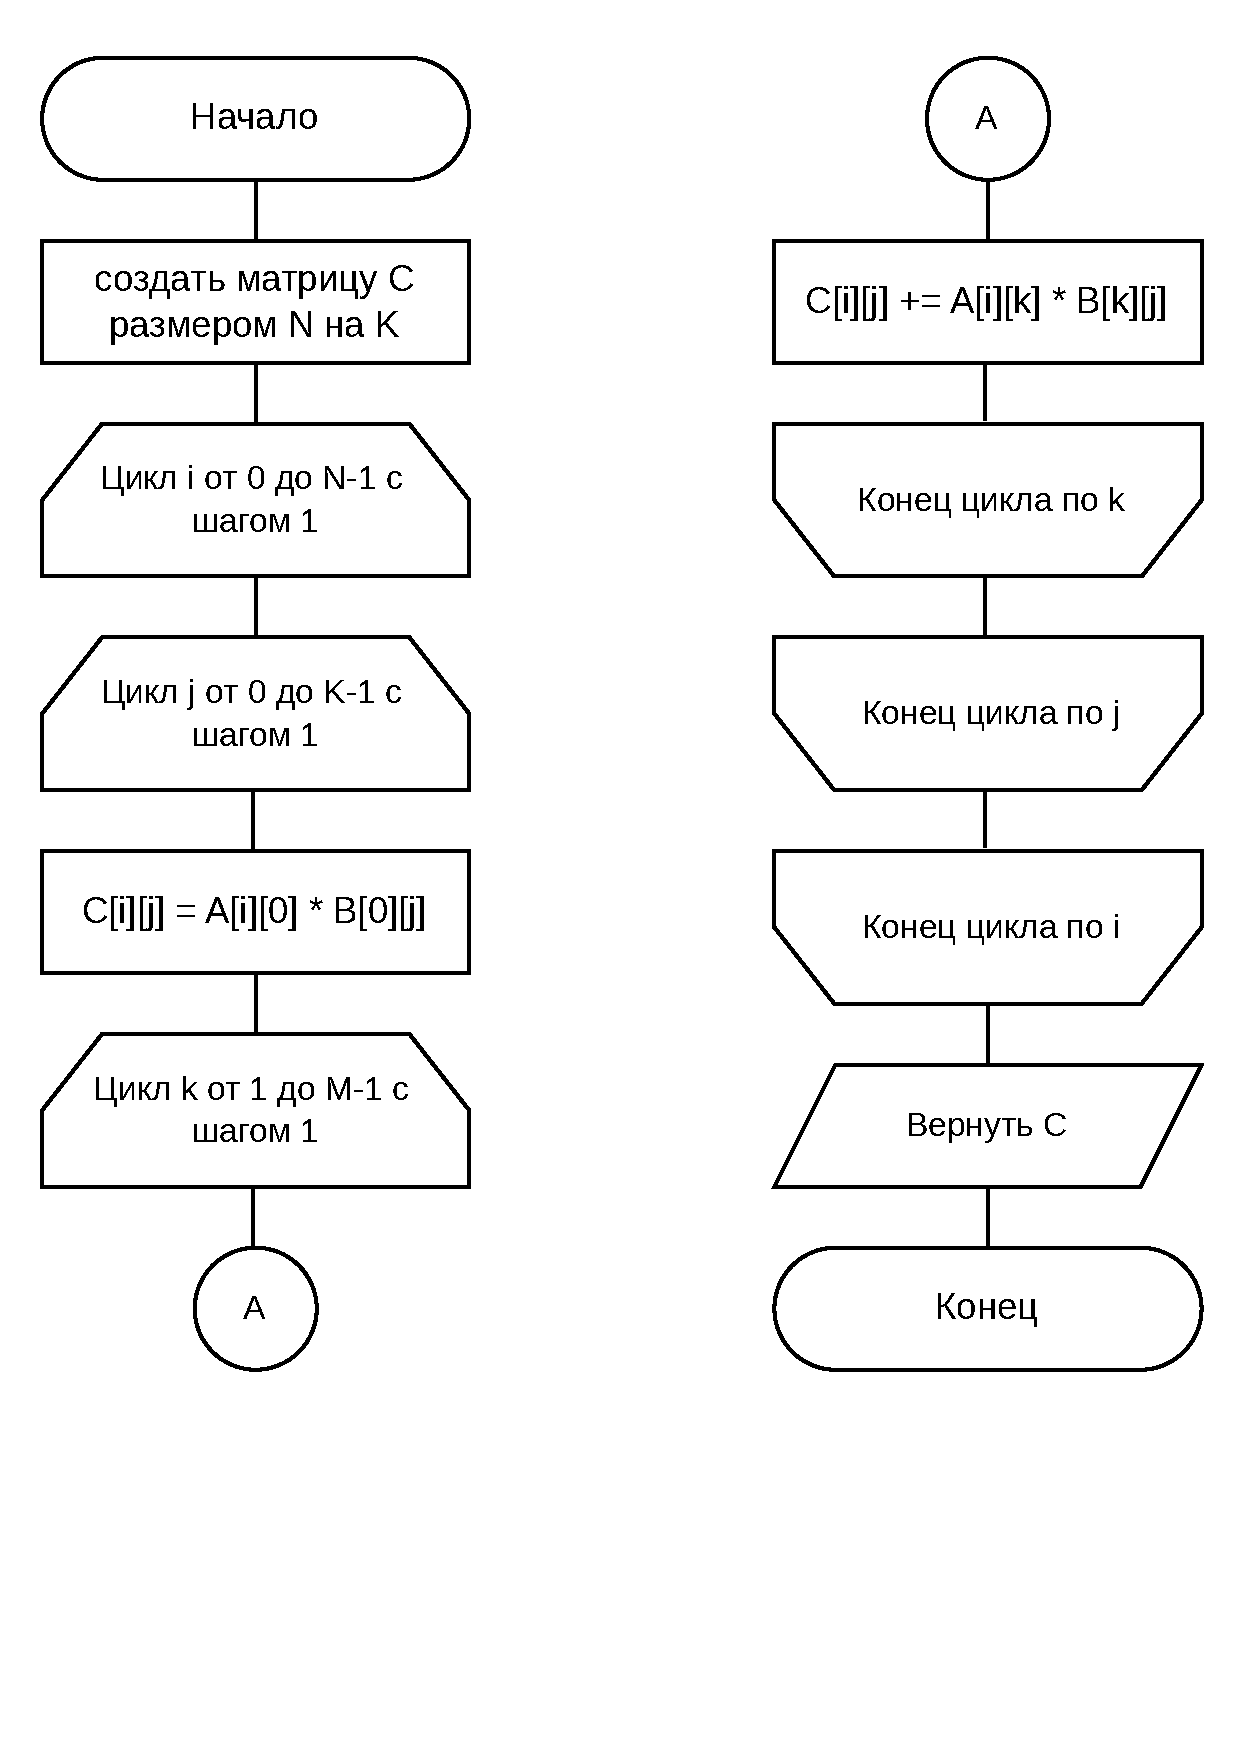
\includegraphics[height=0.8\textheight, width=0.8\textwidth]{tex_parts/scheme2.pdf}
	\caption{\label{fig:sto}Схема стандартного алгоритма нахождения прозведения матриц с оптимизациями}
\end{figure}

\clearpage

\begin{figure}[h!]
	\centering
	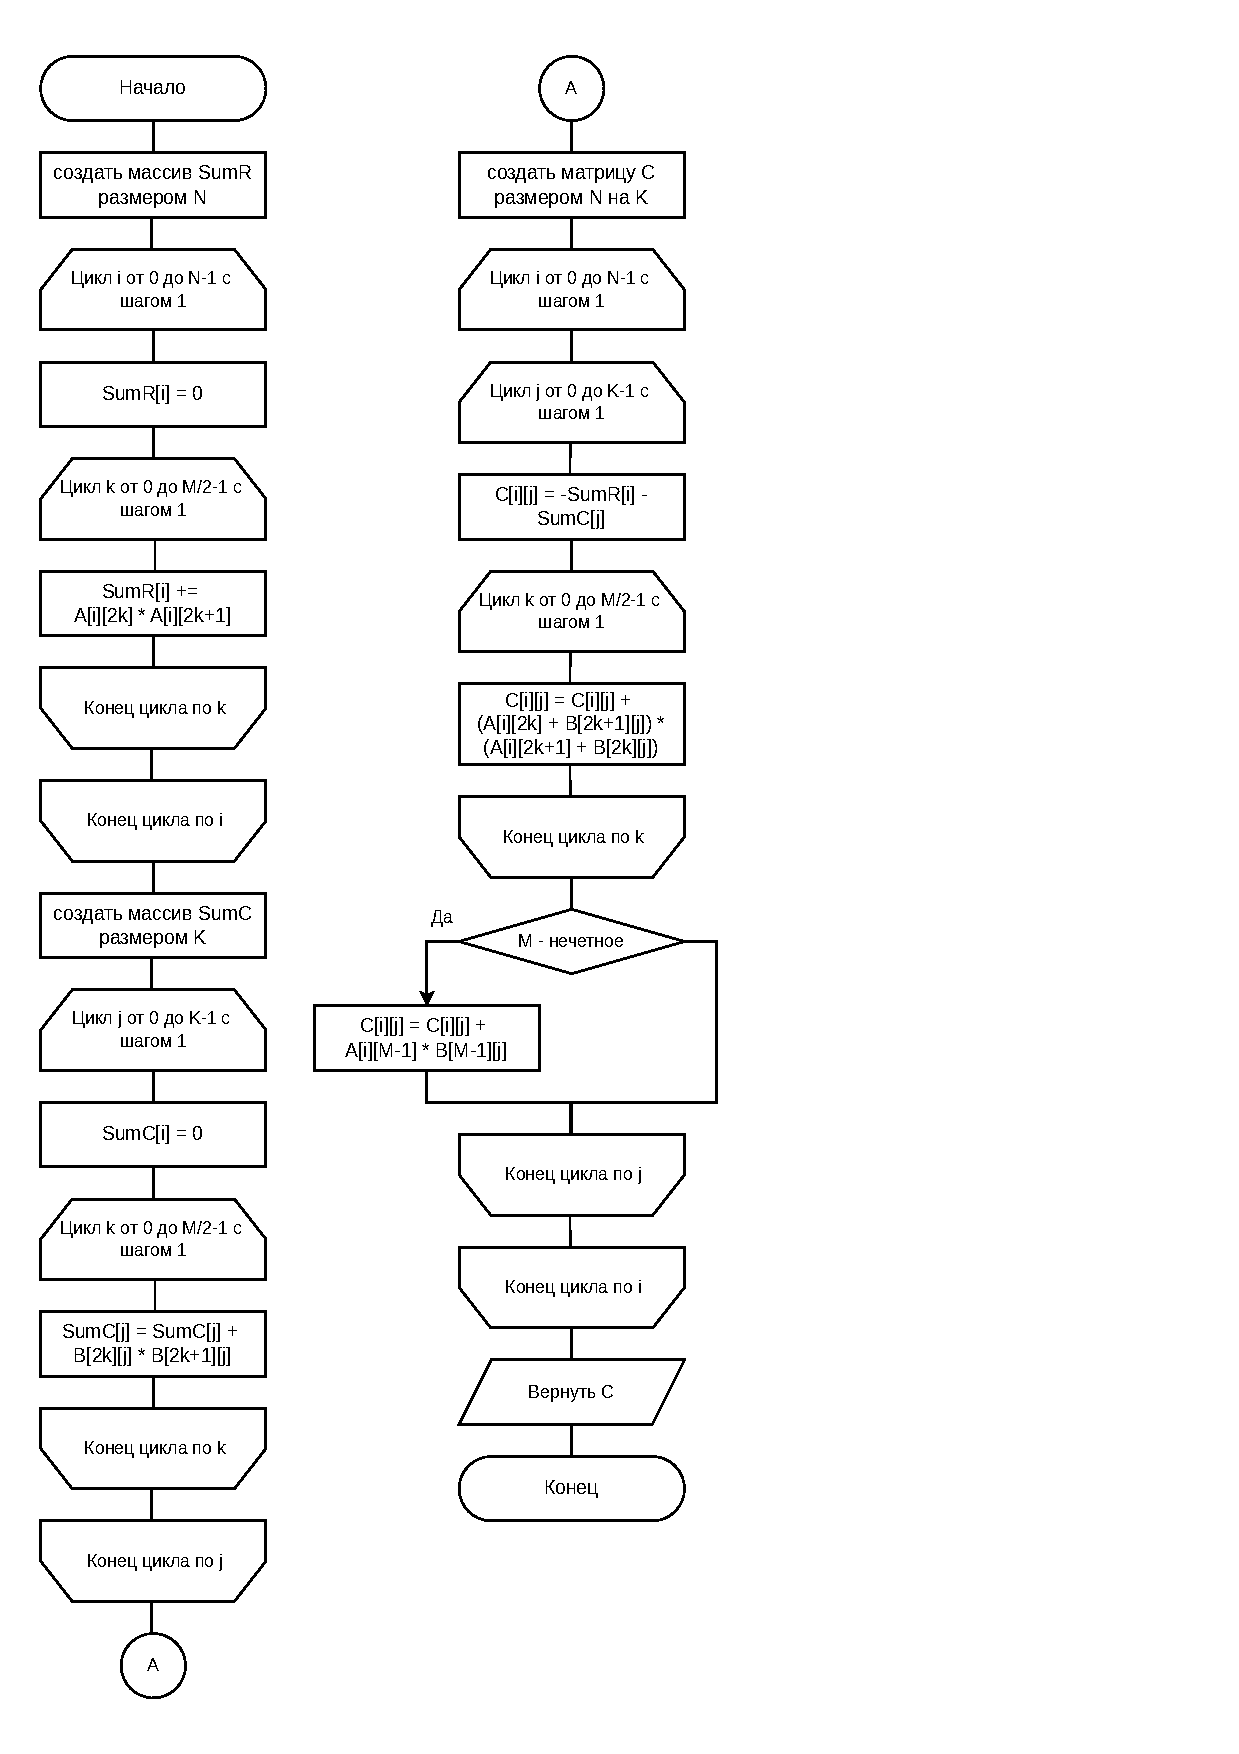
\includegraphics[height=0.8\textheight, width=0.8\textwidth]{tex_parts/scheme3.pdf}
	\caption{\label{fig:vi}Схема алгоритма Винограда}
\end{figure}

\clearpage

\begin{figure}[h!]
	\centering
	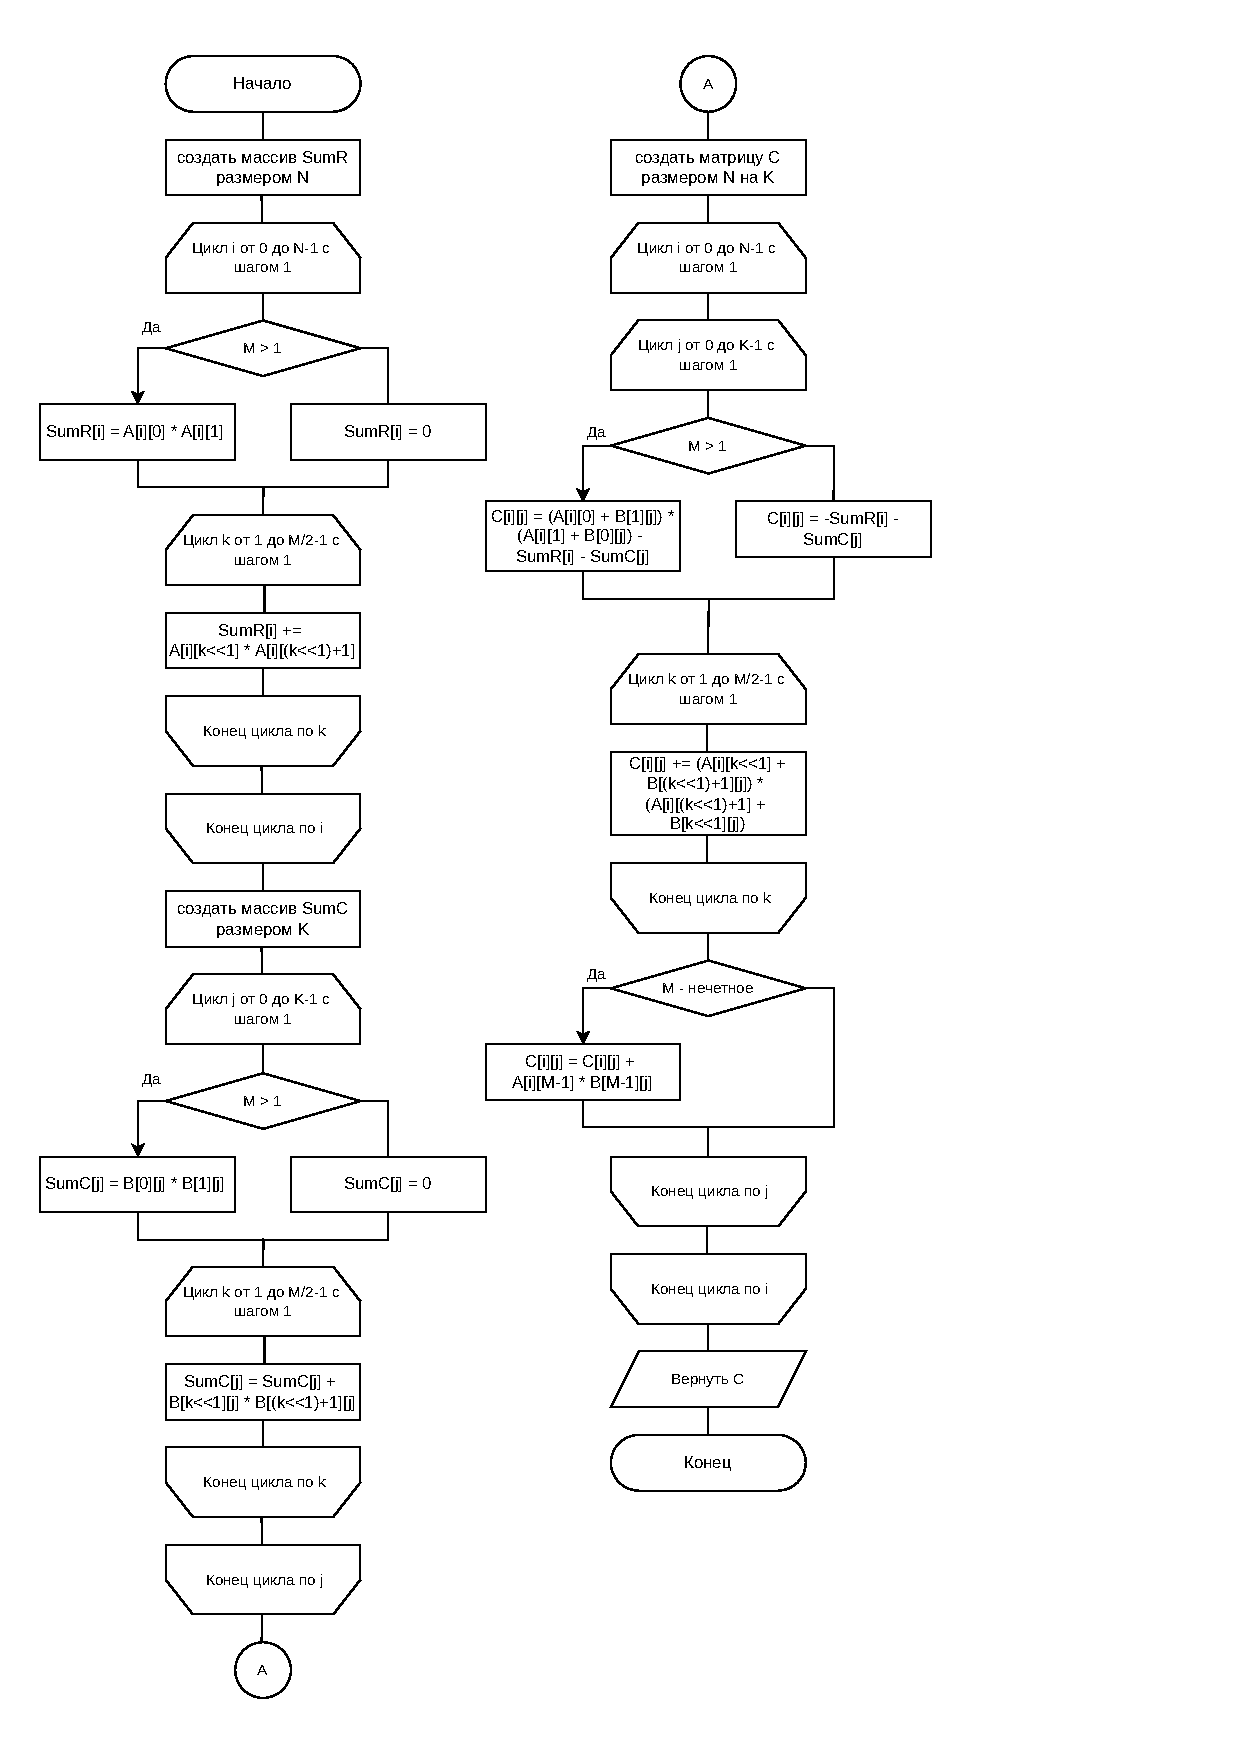
\includegraphics[height=0.8\textheight, width=0.8\textwidth]{tex_parts/scheme4.pdf}
	\caption{\label{fig:vio}Схема алгоритма Винограда с оптимизациями}
\end{figure}

\clearpage

\section{Используемые типы и структуры данных}

При реализации алгоритмов использованы следующие структуры данных:

\begin{itemize}
	\item матрица -- двумерный массив целых чисел.
\end{itemize}

\section{Выводы}

В данном разделе были построены схемы алгоритмов и выбраны структуры данных.

